% !TeX spellcheck = en_US
\documentclass[skip,a4paper]{article}

\usepackage[english]{babel}

\def\subject{CV Olivier CHURLAUD}
\def\title{CV Olivier CHURLAUD}
\def\author{Olivier CHURLAUD}

\usepackage{ucs}
\usepackage[utf8x]{inputenc}
\usepackage[T1]{fontenc}
\usepackage{amsmath}
\usepackage{amsfonts}
\usepackage{amssymb}
\usepackage[top=1cm,bottom=1cm,right=2cm,left=1cm]{geometry}
\usepackage{titlesec}
\usepackage{array}
\usepackage{enumitem}
%% URLs
\usepackage{hyperref}
\usepackage{url}
\usepackage{ulem} % em is underlined

%% Graphics and colors
\usepackage{tikz} % Round corner on picture
\usepackage{color} % enable color
\usepackage{xcolor} % Define own colors
\usepackage{graphicx} % Include picts.

%% Fonts
% cf http://www.tug.dk/FontCatalogue/seriffonts.html
\usepackage[default,osfigures,scale=0.95]{opensans}
% Symbols
\usepackage{marvosym}


%-----Liens PDF-----%
\hypersetup{
	%backref=true, %permet d'ajouter des liens dans...
	%pagebackref=true,%...les bibliographies
	%hyperindex=true, %ajoute des liens dans les index.
	colorlinks=true, %colorise les liens
	breaklinks=true, %permet le retour à la ligne dans les liens trop longs
	urlcolor=black, %couleur des hyperliens
	linkcolor=black, %couleur des liens internes
	%bookmarks=true, %créé des signets pour Acrobat
	%bookmarksopen=true, %si les signets Acrobat sont créés,
	%les afficher complètement.
	pdftitle={\title}, %informations apparaissant dans
	pdfauthor={\author}, %dans les informations du document
	pdfsubject={\subject} %sous Acrobat.
}

\makeatletter

\pagestyle{empty}

\def\UrlFont{\em} % url are `em`, and `em` is underlined with ulem

\titleformat{\section}{\LARGE\bfseries\color{redcv}}{\thesection}{1em}{}[{\titlerule[0.8pt]}]
\titleformat{\subsection}{\normalfont\Large\bfseries}{\thesubsection}{1em}{}

\titlespacing*{\section}{0pt}{2ex plus 0.4ex minus .2ex}{1.3ex plus .2ex}
\titlespacing*{\subsection}{50pt}{2ex plus 0.4ex minus -0.2ex}{0.5ex plus .2ex}

\newcommand{\itemcv}[2]{\textbf{\color{graycv}#1} & #2 \tabularnewline}
	
\newcolumntype{P}[1]{>{\raggedright}p{#1}}
\makeatother	

\makeatletter
	\definecolor{redcv}{HTML}{C5000B}
	\definecolor{graycv}{HTML}{666666}
	\def\scale{0.94}
	\def\descripscale{0.8}
	\def\datescale{0.13}
	\renewcommand{\arraystretch}{1.7}
\makeatother

\begin{document}
\fontsize{8.5}{9.5}
\selectfont

\begin{minipage}[c]{\linewidth}
	\begin{minipage}[c][4cm]{2.6cm}
		~\\~\\
		\begin{tikzpicture}
		\begin{scope}
		\clip [rounded corners=.5cm] (0,0) rectangle coordinate (centerpoint) (2.4,3cm); 
		\node [inner sep=0pt] at (centerpoint) {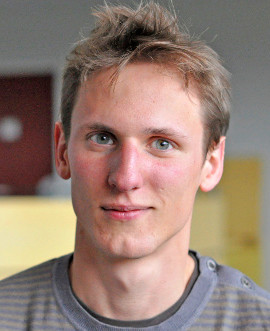
\includegraphics[width=2.4cm]{img/ID_ochurlaud}}; 
		\end{scope}
		\end{tikzpicture}
		\vfill
		~
	\end{minipage}
	\begin{minipage}[c][4cm]{5.5cm}
		\textbf{Olivier CHURLAUD}
		
		\begin{itemize}[itemsep=0.5ex,leftmargin=3ex]
			\footnotesize
			\item[\bfseries @] \url{olivier@churlaud.com}
			\item[\bfseries \color{blue} in] {\scriptsize\url{ fr.linkedin.com/in/olivierchurlaud/}}
			\item[\Telefon] +49 (0)157 52931348
			\item[\Letter] 12, place du grand four \\
			79 370 MOUGON \\ 
			FRANCE
		\end{itemize}
	\end{minipage}
	\begin{minipage}[c][4cm]{10cm}
		\begin{minipage}[c]{7.10cm}
			
\includegraphics[width=6.5cm]{img/ecl}
		\end{minipage}
		\hfill
		\begin{minipage}[c]{2.5cm}
			
\includegraphics[width=2.1cm]{img/tuberlin}
		\end{minipage}
		
		\vfill
		
		\centering
		{
			\setlength{\parskip}{10pt plus 1pt minus 1pt}
			{\LARGE Engineer Student}
			
			{\Large Specialization: Signal and Information processing}
		}
	\end{minipage}
\end{minipage}

\vfill
\begin{minipage}{\linewidth}
	~
	\hfill
	\begin{minipage}{\scale\linewidth}
	~
		\section*{Education}
		\begin{tabular}{p{\datescale\linewidth} P{\descripscale\linewidth}}
			\itemcv{2014 -- 2016}{\textbf{Double degree at TU Berlin: Master Degree Electrical Engineering} \\ Main emphasis: Communication systems, Information theory, Signal processing}
			\itemcv{2012 -- 2016}{\textbf{École Centrale de Lyon: Engineering Degree}} 
			\itemcv{2010 -- 2012}{\textbf{Elite undergrad program}: Lycée Pierre de Fermat in Toulouse (31)\\ Preparation for the competitive entrance examinations to French engineering school
			}
		\end{tabular}
		
		\section*{Experience}
		 
		\begin{tabular}{p{\datescale\linewidth} P{\descripscale\linewidth}}
			\itemcv{2015 -- 2016}{
				\textbf{Master Thesis and Student job at BESSY~II (Berlin, DE)}\\
				Localization and correction of orbit perturbations in BESSY II storage ring. (Signal processing on particle accelerator in Berlin, DE)\\
				\textit{Control theory -- Signal Processing -- C++ Program -- Python -- \textsc{Matlab}}
			}
			\itemcv{2014}{
				\textbf{Research internship with F.~P.~Andriulli (Télécom Bretagne)}\\
				Analysis and design of technics and tools for experiments and computation on EEG material
			}
			\itemcv{2013 -- 2014}{
				\textbf{Research Project: Design of a node connecting WPAN and WLAN networks} \\
				In collaboration with the INL Laboratory (Lyon)\\
				\textit{C Program -- KICAD -- Microcontrollers (Microchip)}
			}
			\itemcv{2012 -- 2013}{
				\textbf{President of the ECLAIR students association} (managed network and IT for more than 700 students) \\
				\textit{Setup of a cloud storage system (based on ownCloud) --  Network Administration -- Design of a meta-website for the students and alumni (Symfony2)}
			}
			\itemcv{~}{
				\textbf{Design of a tool to measure extremely low frequency magnetic fields} \\
				In collaboration with the Ampère Laboratory (Lyon) \\
				\textit{\textsc{Matlab} program -- Setup of a magnetometer on a chip}
			}
			\itemcv{2009 -- 2010}{
				\textbf{Research project in particle physics with CERN and IN2P3} \\
				Received first prize in two science competitions (Olympiades de Physique, Faites de la Science) \\
				\textit{Particle physics -- Experiments -- Popularization -- Design of a board game on the LHC topic}
			}
			\itemcv{2008 -- 2009}{
				\textbf{Writing workshop in partnership with OuLiPo} (Ouvroir de Littérature Potentielle: group of french writers who work by choosing style and content constraints)
			}
		\end{tabular}

		\section*{Professional expertise}
		
		\begin{tabular}{p{\datescale\linewidth} P{\descripscale\linewidth}}
			\itemcv{Management}{Head of project, team coordination, relation with administration}
			\itemcv{Science}{Signal processing, Filter design, Control theory, Electromagnetism, Mathematics, Channel and Source coding}
			\itemcv{Computer Science}{
				Programmation, Machine Learning -- \textbf{Program} Python, C/C++, \textsc{Matlab}, \LaTeX -- \textbf{System and Network administration} Linux, Bridging, VLAN, Virtualization KVM, Apache2
			}
			\itemcv{Languages}{
				\textbf{English}: Fluent, TOEFL 613pts (B2/C1) \\
				\textbf{German} Professional skills: > B2 (European notation system), in Berlin for 2 years
			}
		\end{tabular}
		
		\section*{Interest}
		
		\begin{tabular}{p{\datescale\linewidth} P{\descripscale\linewidth}}
			\itemcv{General \mbox{knowledge}}{
					Literature: Classics from the XIXth and XXth century, Nouveau Roman\\					
					Music, Cinema: French \textit{Cinéma d'auteur} and 40-50s american movies
				}
			\itemcv{Sport}{Mountain sports: Rock climbing, hiking, ski}
			\itemcv{Open Source}{Open source enthusiast, KDE Contributor}
	\end{tabular}
	\end{minipage}
\end{minipage}
\vfill
\end{document}